%%%%%%%%%%%%%%%%%%%%
%%%    INTRO    %%%
%%%%%%%%%%%%%%%%%%%
\documentclass[11pt,fleqn]{article}

\usepackage[utf8]{inputenc}
\usepackage[francais]{babel}
\usepackage{float}
\usepackage{amsmath,amssymb}
\usepackage{tikz}
\usepackage{epigraph}
\usepackage{lipsum}
\usepackage{graphicx}
\usepackage{listings}
\usepackage[T1]{fontenc}
\usepackage{color}
\usepackage[babel=true]{csquotes}

\usepackage[a4paper,margin=3cm,footskip=.5cm]{geometry}

\usetikzlibrary{calc}

\renewcommand{\textflush}{flushepinormal}
\renewcommand\epigraphflush{center}
\renewcommand\epigraphsize{\normalsize}
\setlength\epigraphwidth{0.68\textwidth}

\definecolor{harvardcrimson}{rgb}{0.79,0.0,0.09}
\definecolor{arsenic}{rgb}{0.23,0.27,0.29}
\DeclareFixedFont{\titlefont}{T1}{ppl}{b}{it}{0.5in}


%%%%%%%%%%%%%%%%%%%%%%%
%%%    INTEGRALE    %%%
%%%%%%%%%%%%%%%%%%%%%%%
\newcommand{\deriv}{\mathrm{d}}

%%%%%%%%%%%%%%%%%%%%%%
%%%    CHANCERY    %%%
%%%%%%%%%%%%%%%%%%%%%%
\newcommand*\chancery{\fontfamily{pzc}\selectfont}

%%%%%%%%%%%%%%%%%%%%%%
%%%    PICTURES    %%%
%%%%%%%%%%%%%%%%%%%%%%
\DeclareGraphicsExtensions{.png}
\graphicspath{{Images/}}   

%%%%%%%%%%%%%%%%%%%%%%
%%%    LISTINGS    %%%
%%%%%%%%%%%%%%%%%%%%%%
\lstset{
language=java,
basicstyle=\ttfamily\small, %
identifierstyle=\color{black}, %
keywordstyle=\color{blue}, %
stringstyle=\color{black!60}, %
commentstyle=\it\color{green!95!yellow!1}, %
columns=flexible, %
tabsize=2, %
extendedchars=true, %
showspaces=false, %
showstringspaces=false, %
numbers=left, %
numberstyle=\tiny, %
breaklines=true, %
breakautoindent=true, %
captionpos=b
}
 
\definecolor{codegreen}{rgb}{0,0.6,0}
\definecolor{codegray}{rgb}{0.5,0.5,0.5}
\definecolor{codepurple}{rgb}{0.58,0,0.82}
\definecolor{backcolour}{rgb}{0.95,0.95,0.92}
\lstdefinestyle{mystyle}{
    backgroundcolor=\color{backcolour},   
    commentstyle=\color{codegreen},
    keywordstyle=\color{magenta},
    numberstyle=\tiny\color{codegray},
    stringstyle=\color{codepurple},
    basicstyle=\footnotesize,
    breakatwhitespace=false,         
    breaklines=true,                 
    captionpos=b,                    
    keepspaces=true,                 
    numbers=left,                    
    numbersep=5pt,                  
    showspaces=false,                
    showstringspaces=false,
    showtabs=false,                  
    tabsize=2
} 
 
\lstset{style=mystyle}
\setcounter{tocdepth}{4}
\setcounter{secnumdepth}{4}
\let\EndItemize\enditemize
\def\enditemize{\EndItemize\bigskip}
%%%%%%%%%%%%%%%%%%%%%%%%
%%%    TITLE PAGE    %%%
%%%%%%%%%%%%%%%%%%%%%%%%

\begin{document}

% Drawing definition
\newcommand\titlepagedecoration
{
	\begin{tikzpicture}[remember picture,overlay,shorten >= -10pt]
		\coordinate (aux1) at ([yshift=-15pt]current page.north east);
		\coordinate (aux2) at ([yshift=-410pt]current page.north east);
		\coordinate (aux3) at ([xshift=-4.5cm]current page.north east);
		\coordinate (aux4) at ([yshift=-150pt]current page.north east);

		\begin{scope}[harvardcrimson!75,line width=12pt,rounded corners=12pt]
			\draw
				(aux1) -- coordinate (a)
				++(225:5) --
				++(-45:5.1) coordinate (b);
			\draw[shorten <= -10pt]
				(aux3) --
				(a) --
				(aux1);
			\draw[opacity=0.6,arsenic,shorten <= -10pt]
				(b) --
				++(225:2.2) --
				++(-45:2.2);
		\end{scope}
	
		\draw[arsenic,line width=8pt,rounded corners=8pt,shorten <= -10pt]
			(aux4) --
			++(225:0.8) --
			++(-45:0.8);
	
		\begin{scope}[harvardcrimson,line width=6pt,rounded corners=8pt]
			\draw[shorten <= -10pt]
				(aux2) --
				++(225:3) coordinate[pos=0.45] (c) --
				++(-45:3.1);
			\draw
				(aux2) --
				(c) --
				++(135:2.5) --
				++(45:2.5) --
				++(-45:2.5) coordinate[pos=0.3] (d);   
			\draw 
				(d) -- +(45:1);
		\end{scope}
	
	\end{tikzpicture}%
}

\begin{titlepage}

% Title

\noindent
\titlefont \\\\Systèmes d'exploitation\\Programmation réseaux
\vfill
% Short resume
\epigraph
	{TP 5 - Mise en place d'une architecture client-serveur Java classique avec sécurité logicielle hybride symétrique et asymétrique.}
	% Place & date
	{\textit{Liège, Avril 2015}\\ \textsc{HEPL - Ingénieur Industriel}
	}
\null\vfill
\noindent
\hfill
% Author section
\begin{minipage}{0.5\linewidth}
	\begin{flushright}
		{\large 
			Thibault Reinders\\
			Nassim Rahali\\
			Kaoutare Ahallouch\vspace{20pt}\\
			M 18\vspace{20pt}\\
			Professeur : C. Vilvens
		}
	\end{flushright}
\end{minipage}
% Picture
\begin{tikzpicture}[remember picture,overlay]
	\node[anchor=south west,inner sep=0pt] at ($(current page.south west)+(3cm,4.25cm)$) 
	{
		
\includegraphics[scale=1.2]{logoHEPL}
	};
\end{tikzpicture}
% Author line
\begin{minipage}{0.01\linewidth}
    \rule{1pt}{125pt}
\end{minipage}

\vskip 40pt

\titlepagedecoration

\end{titlepage}

\tableofcontents

\newpage

%%%%%%%%%%%%%%%%%%
%%%    BODY    %%%
%%%%%%%%%%%%%%%%%%

%%%%%%%%%%%%%%%%%%%%%%%%%%%%%%%%%%%%%%%%%%%%%%%%%%%%%%%%
\section{Méthodologique de travail}
Nous nous sommes tout d'abord réparti le travail selon les 3 serveurs à faire (Bank, Data et Web).\\
\begin{itemize}
	\item Bank Server : Thibault
	\item Data Server : Kaoutare
	\item Web Server : Nassim
\end{itemize}
Ensuite, en fonction de l'avancement de chacun dans son serveur, nous avons fait le reste du travail comme suit
\begin{itemize}
	\item Kerberos (AS \& TGS) : Nassim et Thibault
	\item Bank Client : Thibault
	\item Agent Bancaire : Kaoutare et Thibault (chacun la partie utilisant son serveur.)
\end{itemize}
Pour faire les 3 serveurs, nous n'avons pas eut besoin de nous mettre d'accord puisqu'il n'y a pas d'interactions directes entre les différents serveurs, hormis le Web Server qui devait avoir un accès direct aux bases de données des deux autres serveurs.\\\\
Pour l'Agent Bancaire, les interactions entre la partie utilisant le Bank Server et celle utilisant le Data Server n'est pas très importante et nous n'avons pas eut de problème pour développer les 2 en parallèle.\\\\
Pour l'AS et le TGS, il nous a fallu travailler ensemble et communication par communication pour ne pas se tromper dans qui chiffre quoi et avec quelle clé.
%%%%%%%%%%%%%%%%%%%%%%%%%%%%%%%%%%%%%%%%%%%%%%%%%%%%%%%%
\section{Bank Server}
Le serveur a 2 tâches à remplir. Il communique avec les clients Bank Client et Agent Bancaire. On utilise donc 2 \emph{ThreadPoolExecutor} pour qu'un trop grand nombre de clients d'un type ne bloque pas l'autre type de client. Logiquement, on donnera plus de threads au pool destiné à communiquer avec les Banques Clientes qu'à celui pour les Agents Bancaires.\\\\
Le serveur a accès a une base de données \emph{MongoDB} qui contient les banques clientes et leurs demandes d'opérations de crédit et de débit avec notre banque. Typiquement
\begin{lstlisting}
{
	"_id" : 1,
	"type" : "debit",
	"montant" : 1000,
	"valide" : "false",
	"date" : "2015-04-15"
	"banque" : 
	{
		"_id" : 1,
		"name" : "Belfius"
	}
}
\end{lstlisting}
La communication avec les Banques Clientes se fait par SSL, on a donc créé des clés (vérifiées par un CA) enregistrées dans un \emph{keystore}, côté client et côté serveur. Pour ne pas alourdir le code, la création d'une socket SSL a été mise dans un petit jar.\\\\
Par défaut, les demandes de crédit ou de débit des Banques Clientes sont à \emph{false}. Il faudra l'intervention d'un Agent Bancaire pour les valider.\\\\
L'Agent Bancaire peut demander à voir toutes les opérations ou alors les filtrer selon la Banque ou le type d'opération, pour ensuite en sélectionner une ou plusieurs et les valider.
%%%%%%%%%%%%%%%%%%%%%%%%%%%%%%%%%%%%%%%%%%%%%%%%%%%%%%%%
\section{Bank Client}
La Banque Cliente communique donc par SSL avec son serveur. Lors de la connexion, le client doit choisir une banque partenaire de notre banque sous peine d'être refusé. Il peut ensuite faire des demandes de débit et/ou de crédit ou vérifier l'état d'une opération appartenant à sa banque.
\begin{figure}[H]
	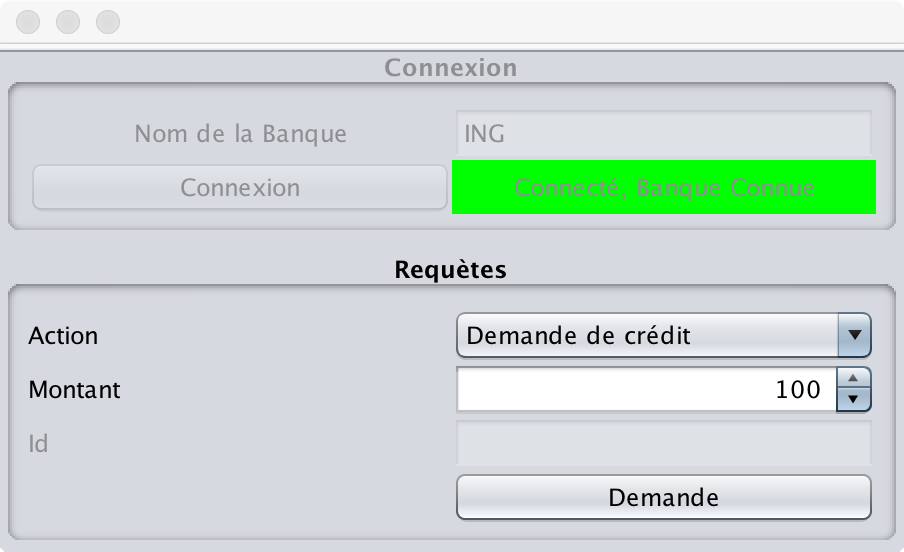
\includegraphics[scale=0.5]{Images/BankClient}
	\centering
	\caption{Application Banque Cliente}
\end{figure}
%%%%%%%%%%%%%%%%%%%%%%%%%%%%%%%%%%%%%%%%%%%%%%%%%%%%%%%%
\section{Agent Bancaire}
\subsection{Vers Bank Server}
L'Agent Bancaire se connecte au Bank Server et s'authentifie au moyen de l'architecture Kerberos. Il peut demander à voir l'ensemble des opérations, ou alors filtrer celles-ci par \emph{Banque} et \emph{Etat}.\\\\
Pour valider une ou plusieurs opérations, l'Agent Bancaire va envoyer la liste des \emph{ids} à valider et le serveur va se charger de faire les updates correspondants sur la base de données.
\begin{figure}[H]
	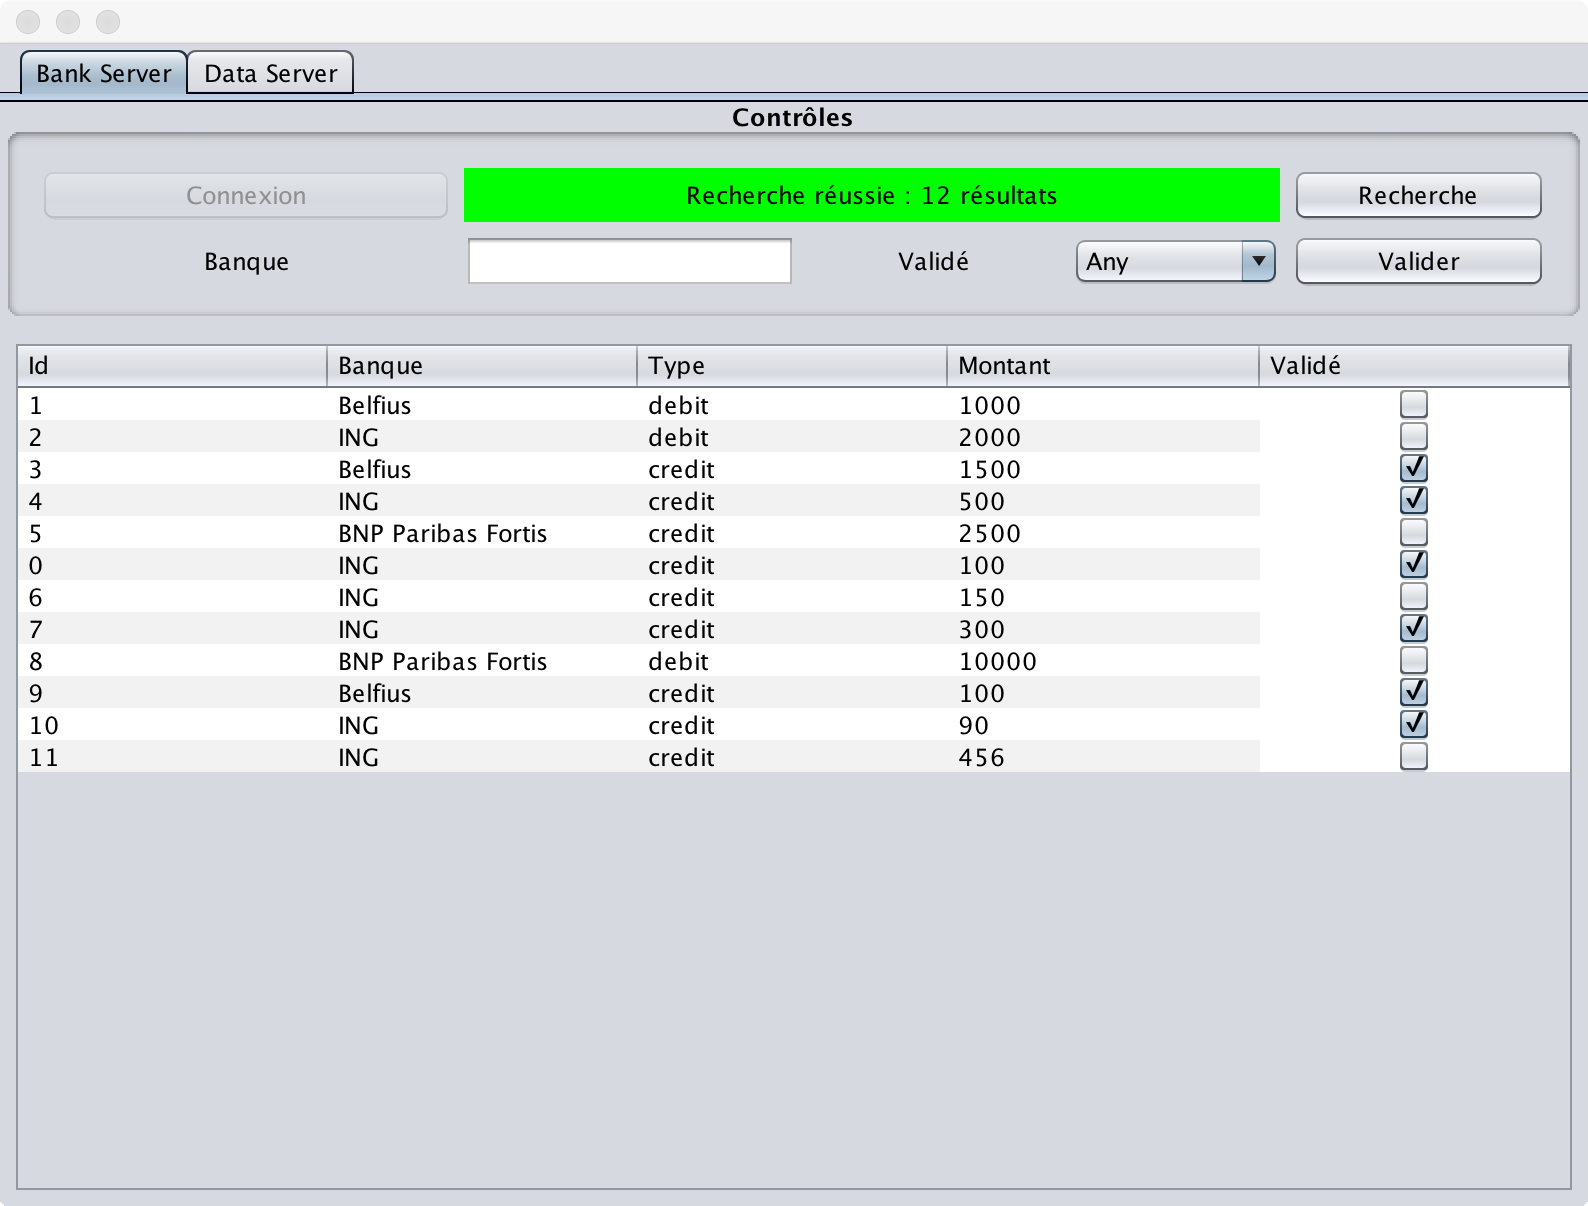
\includegraphics[scale=0.4]{Images/AgentBancaire1}
	\centering
	\caption{Agent Bancaire (Bank Server)}
\end{figure}
\subsection{Vers Data Server}
%% Screen partie 2 %%
%%%%%%%%%%%%%%%%%%%%%%%%%%%%%%%%%%%%%%%%%%%%%%%%%%%%%%%%
\section{Data Server}
%%%%%%%%%%%%%%%%%%%%%%%%%%%%%%%%%%%%%%%%%%%%%%%%%%%%%%%%
\section{Web Server}
%%%%%%%%%%%%%%%%%%%%%%%%%%%%%%%%%%%%%%%%%%%%%%%%%%%%%%%%
\section{AS \& TGS}
C'est la partie qui a été la plus 'délicate' à implémenter. En effet presque toutes les applications de l'architecture sont impactées et il faut travailler en groupe et étape par étape pour être sûr de ne pas chiffrer la mauvaise information ou avec la mauvaise clé pour que le suivant puisse bien décrypter les données.\\\\
Point de vue technique, on notera juste l'utilisation de \emph{SealedObject} pour encapsuler des objets chiffrés puisqu'on ne peut pas simplement crypter un objet et en récupérer les bytes.
%%%%%%%%%%%%%%%%%%%%%%%%%%%%%%%%%%%%%%%%%%%%%%%%%%%%%%%%


\end{document}